\section{Introduction}
\label{sec:intro}
Personal Relationship is an implicit but important feature underlying all dialogues, 
shaping how language is used and perceived during communication. 
%The language content of dialogue is mutually correlated with social relationship between the speakers~\cite{flover}.
Though maybe unconsciously, people start to practice such style 
shifting in communication at very early stage. Study~\cite{mind-reading} finds 
that when children listen to another person, their understanding of the 
counterpart depends on nature of their relationship to the speaker.  
%(in that experiment, 3 kinds of relationships 
%are involved: mother, siblings, and friends). 
Study~\cite{conversational-motive} also finds that conversations between 
different partners are executed under different interpersonal motives, 
and thus the dialogues differ in topics and styles. 
On the other hand, on hearing dialogues from tv/radio shows or life scenes,
audience/overhearers can resort to their communication experiences and commonsense
knowledge to make inference about the speakers relationship, and then further
make sense of the background stories~\cite{FSC}. With computational approaches, we can
more concretely understand where and how interpersonal style shifting happens. It can also help
with computational dialogue understanding at pragmatics level: Similar expressions
may reflect different interpersonal motives, emotions and attitudes between different
relationships. Besides the theoretical interest,
our dataset and methodology can help with future research and applications in related field. 
An automatic relationship classification system can help 
social psychologists prepare large-scale data. For speech-based
cognitive monitoring devices used in mental disorder treatment~\cite{bopolar-monitor, cog-load, tension-monitor}, automatic relationship
classification can help record and understand where the interpersonal stress/stimuli comes from. 
Also it can be used to construct relationship networks for movies and tv shows, 
which is an important but missing from existing movie/tv-show databases 
such as IMDb, TMDb\footnote{\url{https://www.themoviedb.org/}} and 
OMDb\footnote{\url{http://www.omdbapi.com/}}.


\begin{figure}[t!]
	\centering
	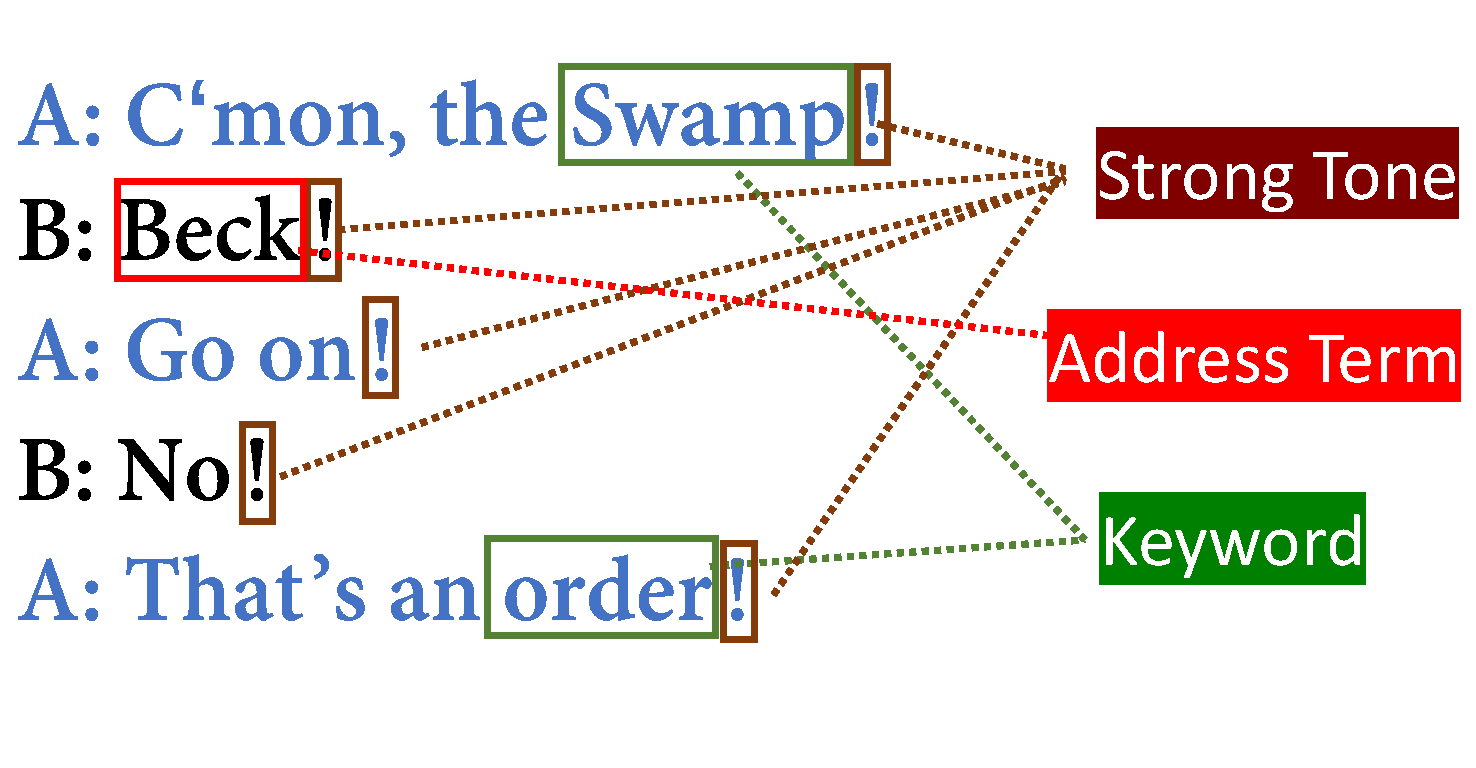
\includegraphics[width=0.85\columnwidth]{instinct.pdf}
	\caption{A sample \textbf{workplace} dialogue and parts that are 
reported as informative by human testers. }
	\label{fig:instinct}
\end{figure}
To study this problem, we first create a dataset of 6307 dyadic dialogue 
sessions (averaging 8.44 turns per session) from movies scripts with relationship labels annotated by humans. 
Movie dialogues, as ``canonical approximation of spontaneous 
talk in interaction''~\cite{canonical}, are found to be 
consistent with naturally occurring ones under stylistic analysis~\cite{FSC}, and the 
overhearer's cognitive process while listening to movie dialogue and real ones
are generally parallel~\cite{overhearer}. We extracted continuous
dialogues that happened between 2 speakers without scene shifting or interrupted
by a third person. 
\figref{fig:instinct} shows a 5-turn dialogue example from our dataset. 
We can see that it's hard to fully contextualize such short segment 
without background knowledge even for humans.
Relationship inference is doable but not straight-forward. 
It involves much commonsense reasoning and sometimes guesswork. 
Although more fine-grained labels are obtained for
future research, in this paper we focus on the family/workplace binary classification 
problem because (1) The definition of family/workplace relationships are clear, relatively
stable and usually don't overlap; (2) Preliminary human performance survey shows that human 
have stable performance (81.69\% Accuracy, 77.5\% Kappa) on the binary classification task, 
while unable to make more detailed inference within such short context; 
(3) our approach can be easily expanded to more categories according to potential application scenario.

%In preliminary tests conducted by human volunteers, we find that 
%the 13-category classification task is hard
%($39\%$ average accuracy) even for human beings due to the limited length 
%of each dialogue session. We hence focus on a relaxed, family/workplace binary 
%classification problem in this paper, which has 3114 samples in our dataset 
%and \textbf{81.68\% human accuracy}. 

Since this can be viewed as a text classification problem, our first attempt is
neural network approaches which boast state-of-the-art performance on many text classification tasks in recent years. These
include character-level convolutional networks (CNN)~\cite{cnn}, 
recurrent neural networks based on long short-term memory (LSTM)~\cite{lstm} 
and hierarchical attention networks~\cite{hierarchy}. 
None of these complex models performs well (see \secref{sec:eval}) due to the limited size and 
heterogeneity of the dataset. 
%given the wide range of topics, intentions and attitudes that can appear in movie dialogues, our dataset doesn't provide enough samples for the networks to learn clear, stable rules. \textcolor{red}{[could add classic relationship extraction methods]} 
To this end, we believe the solution to this {\em small data} learning problem
lies in manually crafted features particular designed to mimic human's 
inference process. 

\citeauthor{flover}~\shortcite{flover} states in a previous study that rules of 
language at the phonemic and morphophonemic levels should be highly stable across 
relationship types, but the lexical, syntactic, and pragmatic levels of language are 
strongly affected by social context. To get a more concrete idea about the 
context-variant parts, we pose this task to human volunteers and 
survey them about 
what they find helpful in their inference process. 
The survey shows that there are numerous factors. 
Take the dialogue session in \figref{fig:instinct} as an example.
Constant use of exclamation points indicate strong tone, 
which makes them sound like arguing.
From the nickname address term ``Beck'' and the phrase ``come on'', 
we infer the two speakers are familiar with each other. 
The mention of ``order'' is very indicative of a work relationship with 
disparity in ranking... 
Generally speaking, both informational indicators and sentimental 
hints are taken into account.
% \KZ{I think you are being too detailed here. Some of the followings can be
%moved to approach. You use the figure to illustrate 1) how difficult the problem
%is and 2) some indicative features. But you can talk rather 
%superficially here.} %Basically, an informative address term such as "dad", "sir" will immediately make things clear. There are also certain topics, or keywords, that provide much certainty. For example, two people talking about kitchen utensils and dinner are likely family members, and if we find "authentication", "report" and "office" in the dialogue, a work place picture emerges in our minds. Without those informative words, we observe tones, which can be reflected by punctuatiosn, modals, sentence types and so on. A higher level of comprehension is based on common sense. Take the sample in figure \ref{fig:instinct}: by asking "Will your father like me", we can infer that the speaker is about to meet his/her lover's family members and seems worried. 
% Achieving such kind of common sense inference ability is actually a very challenging task for artificial intelligence researchers.

In this paper, we define {\em multiple features} corresponding to 
those observations, and provide {\em a set of tools} to extract and vectorize them 
automatically, such as an address term identification tool, 
which achieves a 92.15\% match with human labellers on 
917 sentences, and a sentence type recognizer which is able to 
identify certain linguistic patterns such as disjunctive questions, 
imperatives and entrainment. We feed our new features along with 
other previously studied features in related field,  
such as Linguistic Inquiry and Word Counts (LIWC)~\cite{liwc}, into 
Logistic Regression classifier, and achieve very reasonable accuracies on 
the binary classification problem. 
What's more, by analysing the results, we have some interesting 
findings, e.g., First person and second person pronouns (i,e,. I, you, we) indicate
higher possibility of workplace dialogues than family ones, as well as functional 
words and punctuations. 
More about our experiments, features and results are introduced in \secref{sec:eval}. 




In sum, this paper makes the following contributions:
\begin{itemize}
\item we create the first-ever cross-domain dialogue-to-relationship dataset 
for future study (\secref{sec:data});
\item we propose a simple but effective framework to computationally predict
personal relationships from short dialogues (\secref{sec:method});
\item experiments show that our proposed features, together with the 
classification model achieve $78.49\%$ accuracy on the binary classification
problem, very close to the human performance of $81.68\%$ (\secref{sec:eval});
\item we discover several interesting signals which are not consciously
noticed by humans but very helpful in classification (\secref{sec:method}).
\end{itemize}

